\section{Optical pre-processing}\label{sec:optpreproc}

This section present various pre-processing tasks that can be done
using \app or \mont. The tasks are presented in their classical order
in which they can be chained to obtain a calibrated, pan-sharpened 

\subsection{Optical radiometric calibration}\label{ssec:optcal}

In remote sensing imagery, pixel values are called DN (for Digital
Numbers) and can not be physically interpreted and compared: they are
influenced by various factors such as the amount of light flowing
trough the sensor, the gain of the detectors and the analogic to
numeric converter.

Depending on the season, the light and atmospheric conditions, to
position of the sun or the sensor internal parameters, these DN can
drastically change for a given pixel (apart from any ground change
effects). Moreover, these effect are not uniform over the spectrum:
for instance aerosol amount and type has usually more impact on the
blue channel.

Therefore, it is necessary to calibrate the pixel values before any
physical interpretation is made out of them. In particular, this
processing is mandatory before any comparison of pixel spectrum
between several images (from the same sensor), and to train a
classifier without dependence to the atmospheric conditions at the
acquisition time.

Calibrated values are called surface reflectivity, which is a ratio
denoting the fraction of light that is reflected by the underlying
surface in the given spectral range. As such, its values lie in the
range $[0,1]$. For convenience, images are often stored in thousandth
of reflectivity, so that they can be encoded with an integer type.
Two levels of calibration are usually distinguished:

\begin{itemize}
\item The first level is called \emph{Top Of Atmosphere (TOA)}
  reflectivity. It takes into account the sensor gain, sensor spectral
  response and the solar illumination.
\item The second level is called \emph{Top Of Canopy (TOC)}
  reflectivity. In addition to sensor gain and solar illumination, it
  takes into account the optical thickness of the atmosphere, the
  atmospheric pressure, the water vapor amount, the ozone amount, as
  well as the composition and amount of aerosol gasses.
\end{itemize}

This transformation can be done either with \app or with
\mont. Sensor-related parameters such as gain, date, spectral
sensitivity and sensor position are seamlessly read from the image
metadata. Atmospheric parameters can be tuned by the user. Supported
sensors are :
\begin{itemize}
\item SPOT5,
\item QuickBird,
\item Ikonos,
\item WorldView1,
\item WorldView2,
\item Formosat.
\end{itemize}

\subsubsection{Optical calibration with \app}

The \application{otbOpticalCalibration-cli} application from \app
allows to perform command-line optical calibration. The mandatory
parameters are the input and output images and the level of
calibration (either TOA or TOC). All other parameters are
optional. The output images are expressed in thousandth of
reflectivity using a 16 bits unsigned integer type.

A basic TOA calibration task can be performed with the following command :

\begin{verbatim}
otbOpticalCalibration-cli -in  input_image -out output_image -level TOA
\end{verbatim}

A basic TOC calibration task can be performed with the following command :

\begin{verbatim}
otbOpticalCalibration-cli -in  input_image -out output_image -level TOC
\end{verbatim}

\subsubsection{Optical calibration with \mont}

These transformations can also be done in \mont.

The 6S model needs atmospheric parameters to be able to compute
radiative terms to estimate the atmoshperic contributions on the input
signal. Default parameters are available in the module.  For
atmospheric parameters, it is possible to indicate AERONET file. The
AERONET (AErosol RObotic NETwork) program is a federation of
ground-based remote sensing aerosol networks established by NASA and
PHOTONS (Univ. of Lille 1, CNES, and CNRS-INSU) and is greatly
expanded by collaborators from national agencies, institutes,
universities, individual scientists, and partners. The program
provides accessible public domain database of aerosol optical,
mircrophysical and radiative properties.

The module produce four outputs:

\begin{itemize}
\item Luminance image
\item TOA reflectance image
\item TOC reflectance image
\item Difference TOA-TOC image which allows to get the estimation of atmospheric contribution
\end{itemize}

\begin{figure}
  \center
  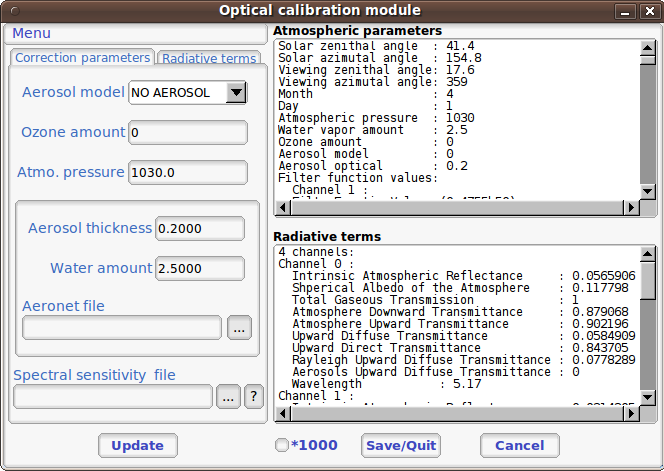
\includegraphics[width=0.6\textwidth]{../Art/MonteverdiImages/monteverdi_optical_calibration.png}
  \itkcaption[GUI of the optical calibration module based on the 6S model]{Optical calibration module.}
  \label{fig:opticalcalibration}
\end{figure}


\begin{figure}
  \center
  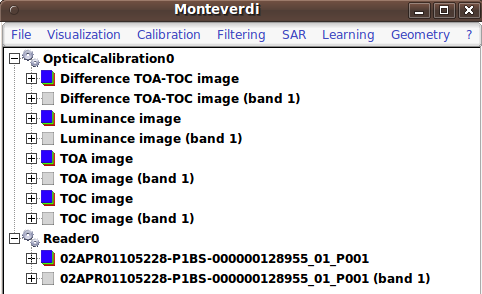
\includegraphics[width=0.6\textwidth]{../Art/MonteverdiImages/monteverdi_optical_calibration_outputs.png}
  \itkcaption[Output of the optical calibration module]{Optical calibration module's outputs.}
  \label{fig:opticalcalibrationoutput}
\end{figure}

\subsection{Pan-sharpening}\label{ssec:pxs}

Because of physical constrains on the sensor design, it is difficult
to achieve high spatial and spectral resolution at the same time : a
better spatial resolution means a smaller detector, which in turns
means lesser optical flow on the detector surface. On the contrary,
spectral bands are obtained through filters applied on the detector
surface, that lowers the optical flow, so that it is necessary to
increase the detector size to achieve an acceptable signal to noise
ratio.

For these reasons, many high resolution satellite payload are composed
of two sets of detectors, which in turns delivers two different kind
of images :

\begin{itemize}
\item The multi-spectral (XS) image, composed of 3 to 8 spectral bands
  containing usually blue, green, red and near infra-red bands at a
  given resolution (usually from 2.8 meters to 2 meters).
\item The panchromatic (PAN) image, which is a grayscale image acquired by a
  detector covering a wider part of the light spectrum, which allows
  to increase the optical flow and thus to reduce pixel
  size. Therefore, resolution of the panchromatic image is usually
  around 4 times lower than the resolution of the multi-spectral image
  (from 46 centimeters to 70 centimeters).
\end{itemize}

It is very frequent that those two images are delivered side by side
by data providers. Such a dataset is called a bundle. A very common
remote sensing processing is to fuse the panchromatic image with the
multi-spectral one so as to get an image combining the spatial
resolution of the panchromatic image with the spectral richness of the
multi-spectral image. This operation is called pan-sharpening.

This fusion operation requires two different steps :
\begin{enumerate}
\item The multi-spectral (XS) image is zoomed and registered to the
  panchromatic image,
\item A pixel-by-pixel fusion operator is applied to the co-registered
  pixels of the multi-spectral and panchromatic image to obtain the
  fused pixels.
\end{enumerate}

Using either an application from \app or modules from \mont, it is
possible to perform both steps in a raw, or step-by-step fusion, as
described in the above sections.

\subsubsection{Pan-sharpening with \app}

The \application{otbBundleToPerfectSensor-cli} application allows to
perform both steps in a raw. Seamless sensor modelling is used to
perform zooming and registration of the multi-spectral image on the
panchromatic image. Then, a simple pan-sharpening is applied,
according to the following formula:

\begin{equation}
PXS(i,j) = \frac{PAN(i,j)}{PAN_{smooth}(i,j)} \cdot XS(i,j)
\end{equation}

Where $i$ and $j$ are pixels indices, $PAN$ is the panchromatic image,
$XS$ is the multi-spectral image and $PAN_{smooth}$ is the
panchromatic image smoothed with a kernel to fit the multi-spectral
image scale.

Here is a simple example of how to use the
\application{otbBundleToPerfectSensor-cli} application:

\begin{verbatim}
otbBundleToPerfectSensor-cli -inP pan_image -inXS xs_image -out output_image
\end{verbatim}

There are two more optional parameters that can be useful for this
tool:
\begin{itemize}
\item The $-dem$ option allows to specify a directory containing DEM
  formatted for OTB (see section~\ref{ssec:dem}). Since registration
  and zooming of the multi-spectral image is performed using
  sensor-models, it may happen that the registration is not perfect in
  case of landscape with high elevation variation. Using a DEM in this
  case allows to get better registration (see \ref{ssec:registration}
  to learn about how to lower registration error).
\item The $-lmSpacing$ option allows to specify the step of the
  registration grid between the multi-spectral image and panchromatic
  image. This is expressed in amount of panchromatic pixels. A lower
  value gives a more precise registration but implies more computation
  with the sensor models, and thus increase the computation
  time. Default value is 10 pixels, which gives sufficient precision
  in most of the cases.
\end{itemize}

Pan-sharpening is a quite heavy processing requiring a lot of system
resource. The $-ram$ option allows you to limit the amount of memory
available for the computation, and to avoid overloading your
computer. Increasing the available amount of RAM may also result in
better computation time, seems it optimises the use of the system
resources. Default value is 256 Mb.


\subsubsection{Pan-sharpening with \mont}

\mont allows to perform step-by-step fusion. The followings screenshots highlight operations needed to perform Pan-Sharpening.

\begin{itemize}
\item Open panchromatic and multispectral images in monteverdi using the \mmod{Open Dataset} module or using the  $-iml$ option of the \mont executable.

\item The \mmod{Superimpose} module is used to zoomed and registered
  the multispectral on the panchromatic image. As a result, we get a
  multispectral dataset with the same geographic extension and the
  same resolution as the panchromatic image, cf ~\ref{fig:qbmulsuper}.

\begin{figure}
  \center
  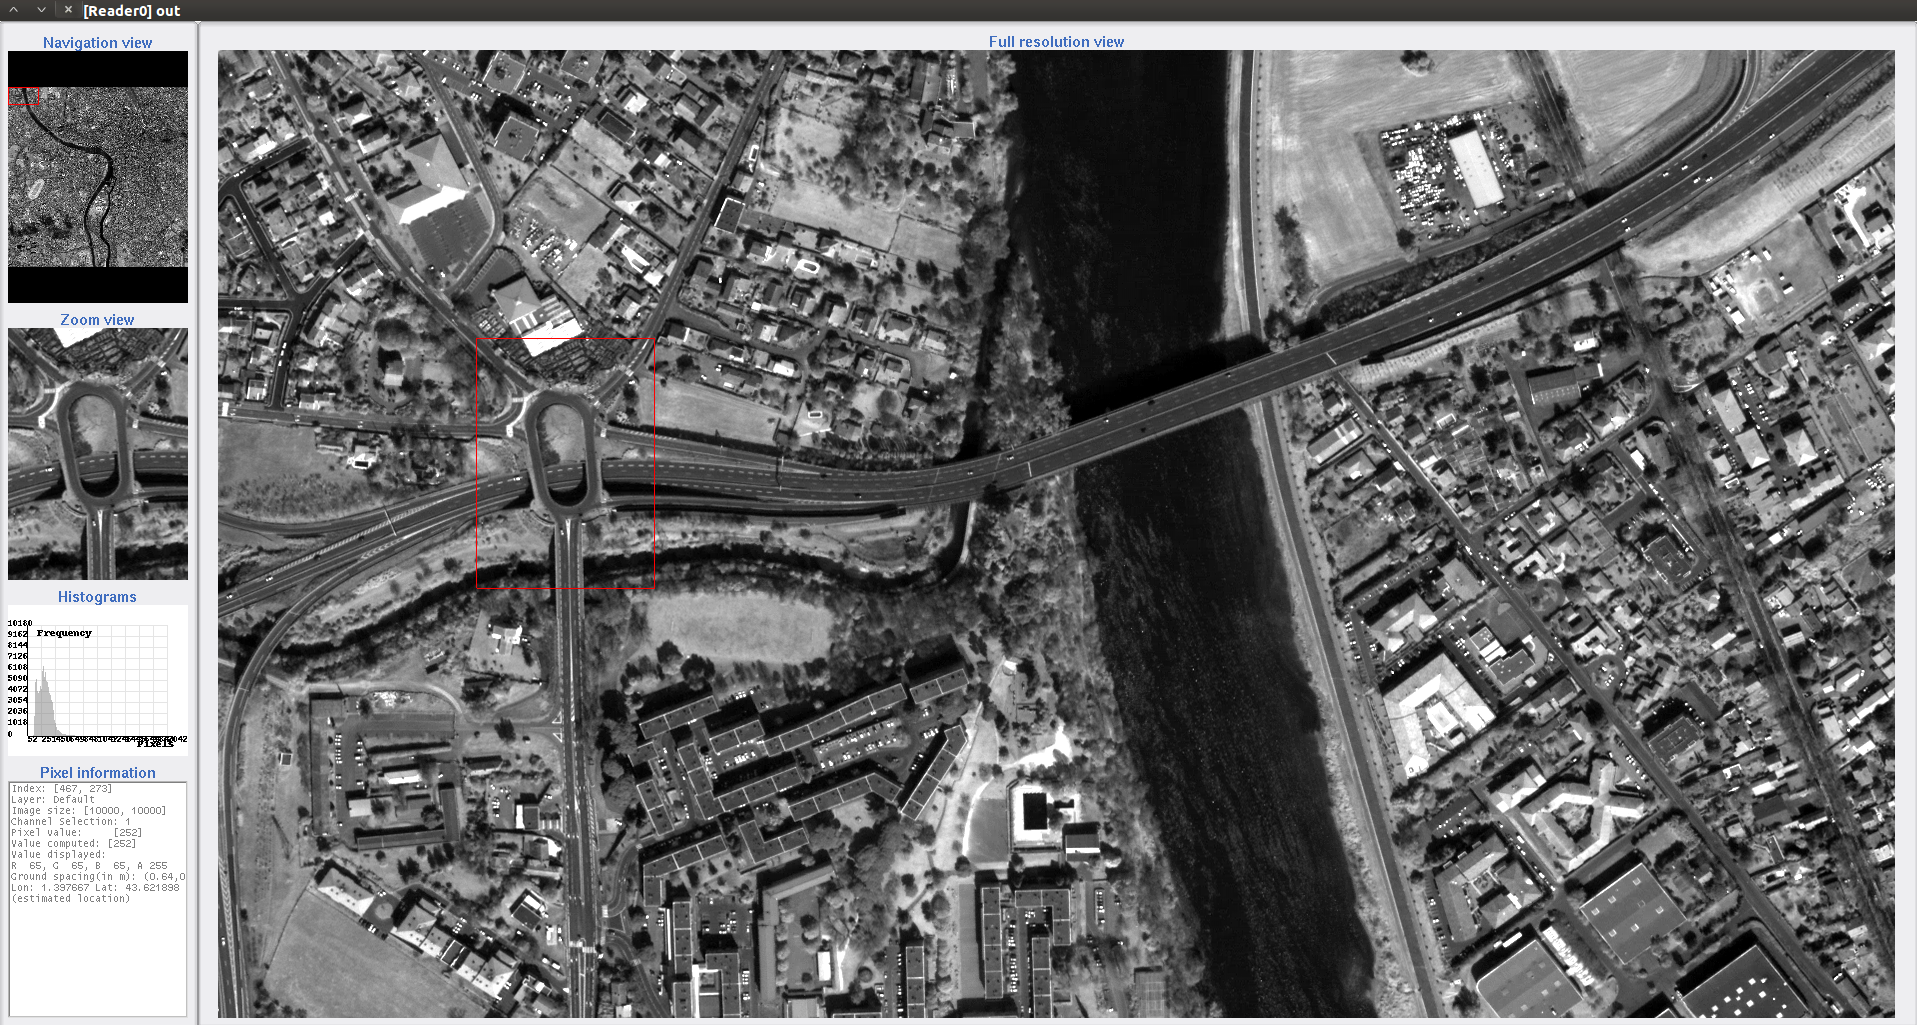
\includegraphics[width=0.45\textwidth]{../Art/MonteverdiImages/monteverdi_QB_PAN_ROI.png}
  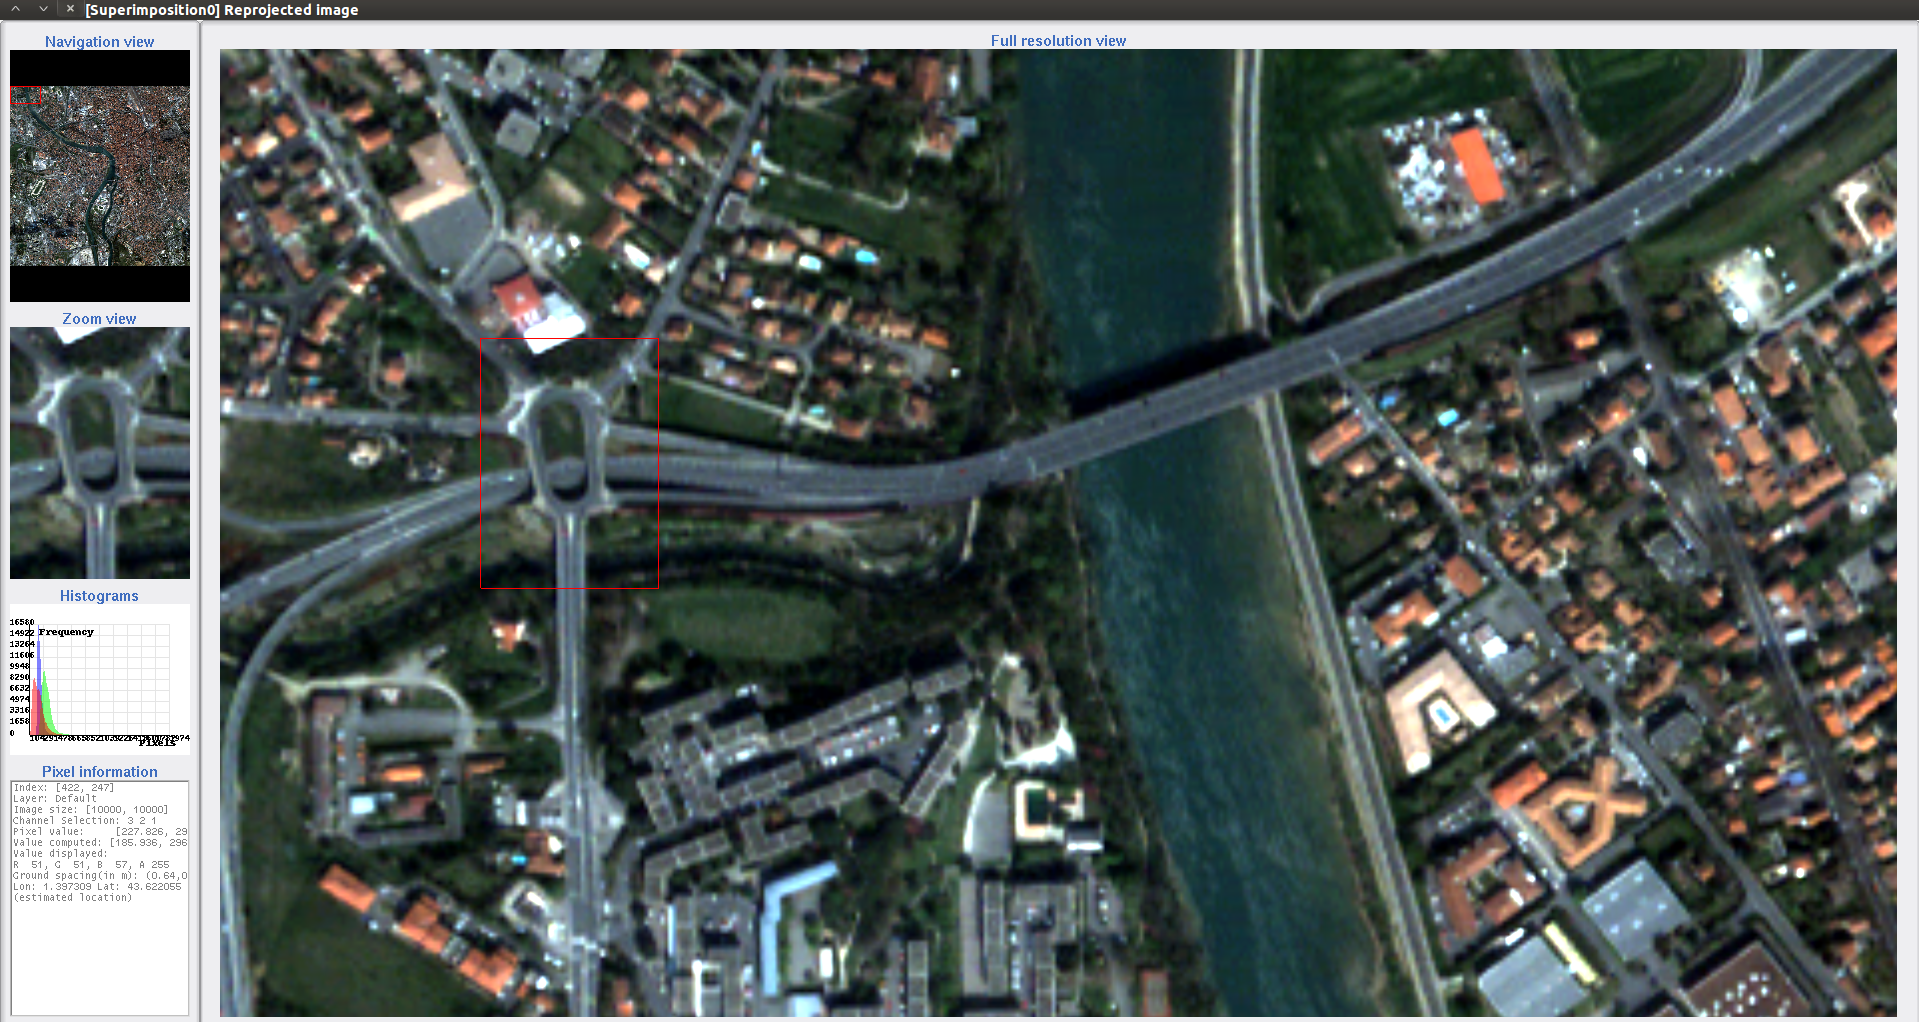
\includegraphics[width=0.45\textwidth]{../Art/MonteverdiImages/monteverdi_QB_MUL_Superimpose.png}
  \itkcaption[Input panchromatic and zoomed and registered multispectral image over it]{Panchromatic and Zoomed and registered Multispectral image.}
  \label{fig:qbmulsuper}
\end{figure}

\item Now the \mmod{Simple RCS pan-sharpening} module can be used using the panchromatic and the multispectral images as inputs. It produces a multispectral image with the same resolution and geographic extension (cf ~\ref{fig:pansharpen}).

\begin{figure}
  \center
  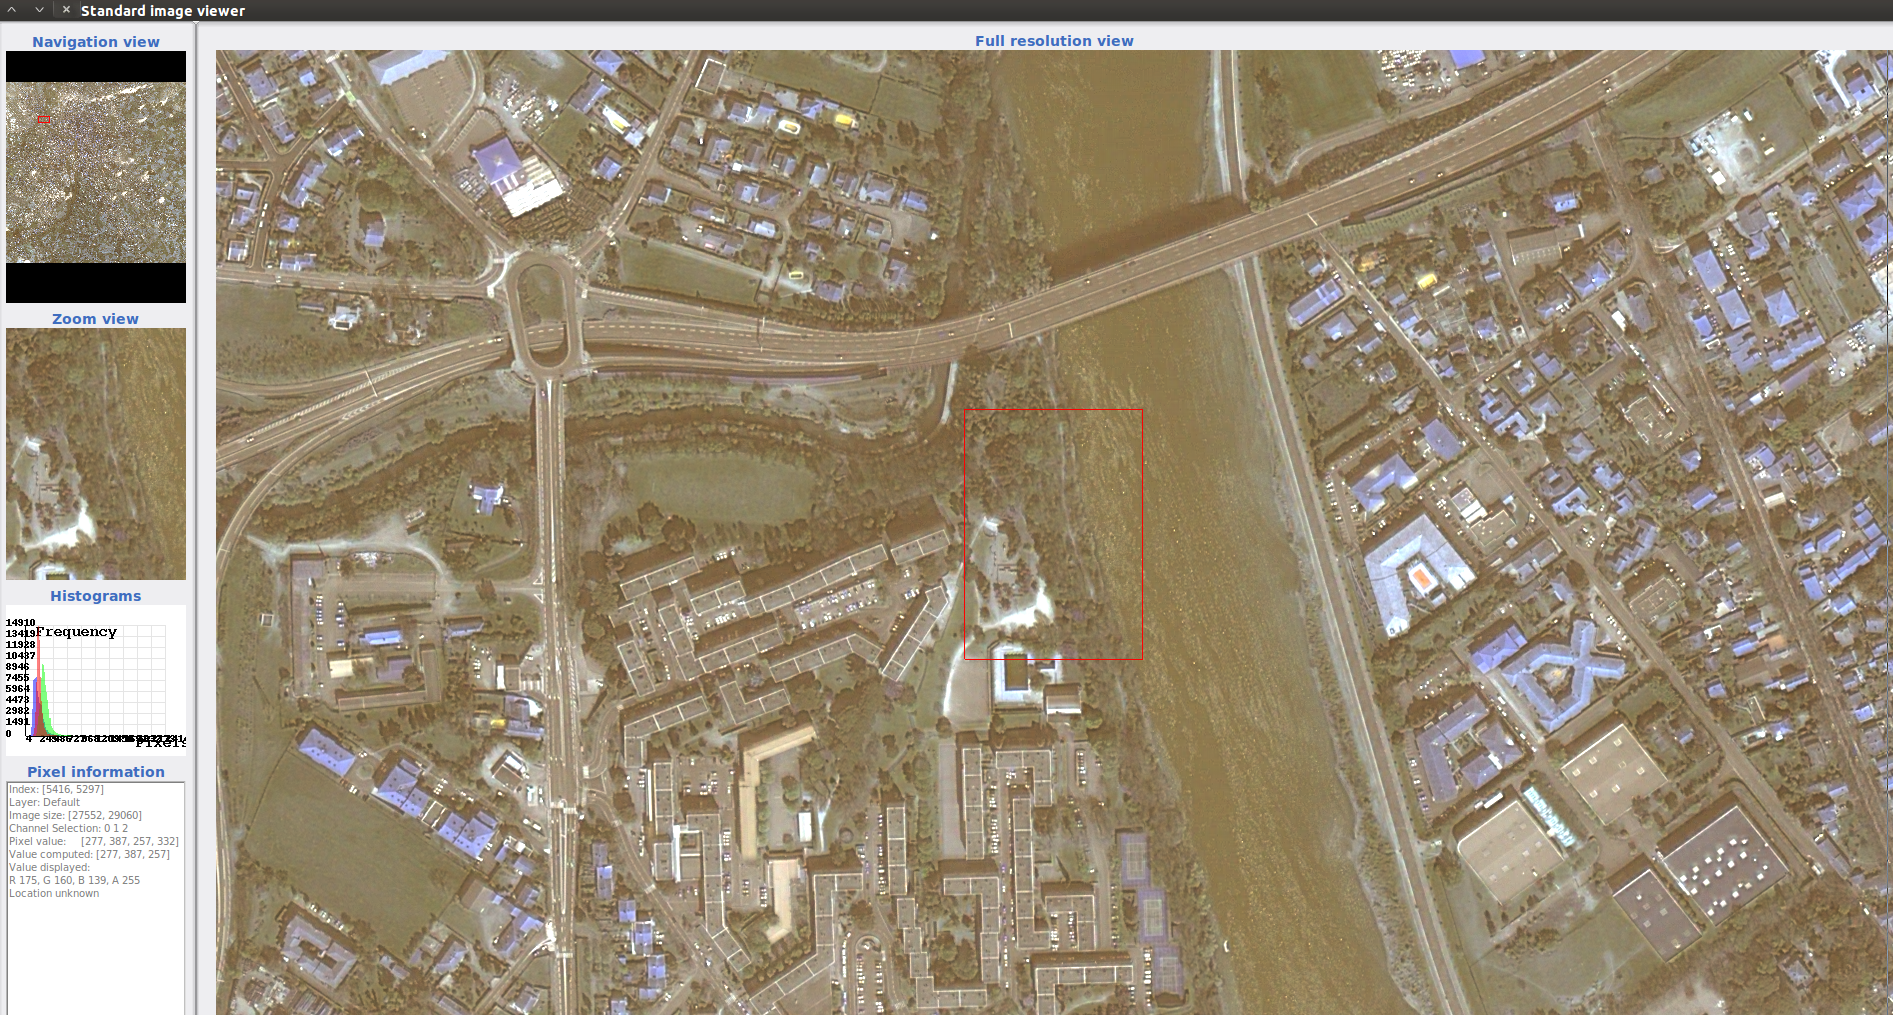
\includegraphics[width=0.6\textwidth]{../Art/MonteverdiImages/monteverdi_QB_XS_pan-sharpened.png}
  \itkcaption[Pan-sharpened image]{Pan-sharpened image using the simple RCS module.}
  \label{fig:pansharpen}
\end{figure}

\end{itemize}


Please also note that since registration and zooming of the
multi-spectral image with the panchromatic image relies on sensor
modelling, this tool will work only for images whose sensor models is
available in \otb (see section~\ref{ssec:ortho} for a detailed
list). It will also work with ortho-ready products in cartographic
projection.

\subsection{Digital Elevation Model management}\label{ssec:dem}

A Digital Elevation Model (DEM) is an georeferenced image (collection
of images) of the elevation. DEM are useful for tasks involving sensor
to ground and ground to sensor coordinate transforms like
ortho-rectification (see section~\ref{ssec:ortho}). In facts, these
transforms need to find the intersection between the line of sight of
the sensor and the earth geo�d. If a simple sphero�d is used as the
earth model, potentially high localisation errors can be made in areas
where elevation is high or perturbed. Of course, DEM accuracy and
resolution have a great impact on the precision of these transforms.

There exists two main available DEM free of charges with worldwide
cover, which are both delivered as  1�-by-1� tiles:
\begin{itemize}
\item \href{http://www2.jpl.nasa.gov/srtm/}{The Shuttle Radar
  topographic Mission (SRTM)} is a 90 meters resolution DEM, obtained
  by radar interferometry during a campaign of the Endeavour space
  shuttle from NASA in 2000. The 
\item The \href{http://www.ersdac.or.jp/GDEM/E/2.html}{Advanced
  Spaceborne Thermal Emission and Reflection Radiometer (ASTER)} is a
  30 meters resolution DEM obtained by stereoscopic processing of the
  archive of the ASTER instrument.
\end{itemize}

The \otb suite relies on \ossim capabilities for sensor modelling and
DEM handling. Tiles of a given DEM are supposed to be located within a
single directory. Whenever some application from \app or module from
\mont requires a DEM, there is an option or a field to set the DEM
directory.

\subsubsection{Making DEM files usable in \otb suite using \app}

Georeferenced files containing elevation data (including file from
SRTM and ASTER) need to be converted to a specific file format before
being compatible with \ossim and \otb. The
\application{otbDEMConvert-cli} application allows to perform this
conversion with the following command:

\begin{verbatim}
otbDEMConvert-cli -in input_image -out output_image
\end{verbatim}

The output image can then be placed in the directory containing DEM
files.

\subsubsection{Extract the DEM image corresponding to your image using
  \mont}


\subsection{Ortho-rectification and map projections}\label{ssec:ortho}

todo.

\subsection{Residual registration}\label{ssec:registration}

todo.
